
\begin{itemize}
\item how do we run ill-typed programs?
\item for a lang like ocaml, dynamic semantics are independent of static
  semantics, just lambda calculus. so no problem to run ill-typed
  program
\item but what about functions? what type of arguments should we pass? consider

\begin{lstlisting}
let f x = 
  let y = 1 + x in
    1. +. y
\end{lstlisting}

does \texttt{f} take an int, float, string? int and float are both
somewhat plausible, but string or anything else is ``clearly'' bogus. so
we cannot provide \emph{completely arbitrary} inputs to
\texttt{f}. Instead, we call \texttt{f} with a \emph{hole}, written
\hole{}, which is a placeholder for a value whose type we have not
yet determined. As we execute the program, we instantiate holes with
concrete values as demanded by the primitive operations in the
program. For example, the hole we pass to f will be instantiated to an
int when we reach the \lstinline{1 + x} term. Thus, y will be an int as
well, and the program will get stuck at \lstinline{1. +. y}. \ES{this
  reads more like overview text..}

Next, we formalize our search for witnesses to type-errors. We present
the syntax and dynamic semantics of a simple lambda calculus with
integers and booleans, extended with our notion of holes, as well as our
search algorithm. We prove that our system \emph{soundly} finds
witnesses, \ie if we find a witness then there is no possible typing for
the input program.

\subsection{Syntax}
\label{sec:syntax}
\begin{figure}
% \hrule width 0.48\textwidth \vspace{0.05in}
$$
\begin{array}{rrcl}
% \emphbf{Configurations} \quad
%   & c & ::=    & \triple{e}{\vsu}{\tsu} \spmid \triple{\stuck}{\vsu}{\tsu} \\[0.05in]

\emphbf{Expressions}
  & \estuck & ::= & e \spmid \stuck \\
  & e & ::=    & v \spmid x \spmid \eapp{e}{e} \spmid \eplus{e}{e}\\
  &   & \spmid & \eif{e}{e}{e} \\
  % &   & \spmid & \elet{x}{e}{e} \\
  &   & \spmid & \epair{e}{e} \spmid \epcase{e}{x}{x}{e} \\
  &   & \spmid & \enode{e}{e}{e} \spmid \eleaf \\
  &   & \spmid & \ecase{e}{e}{x}{x}{x}{e} \\[0.1in]

\emphbf{Values}
  & v  & ::= & n \spmid b \spmid \efun{x}{e} \spmid \vhole{\thole} \spmid tr \\
  & tr & ::= & \vnode{t}{v}{v}{v} \spmid \vleaf{t} \\[0.05in]

\emphbf{Integers}
  & n & ::= &  0,1,-1,\ldots \\[0.05in]

\emphbf{Booleans}
  & b & ::= &  \etrue \spmid \efalse \\[0.05in]

\emphbf{Types}
  & t & ::=     & \tbool \spmid \tint \spmid \tfun \\
  &   &  \spmid & \tprod{t}{t} \spmid \ttree{t} \spmid \thole \\[0.05in]

\emphbf{Substitutions}
  & \vsu & ::= & \emptysu \spmid \extendsu{\vsu}{\vhole{\thole}}{v} \\
  & \tsu & ::= & \emptysu \spmid \extendsu{\tsu}{\thole}{t} \\[0.1in]
% \end{array}
% $$
% % \hrule width 0.48\textwidth
% $$
% \begin{array}{rrcl}
\emphbf{Contexts}
  & C
  & ::=
  &   	 \bullet
  \spmid \eapp{C}{e}
  \spmid \eapp{v}{C} \\
  & & \spmid & \eplus{C}{e} \spmid \eplus{v}{C} \\
  & & \spmid & \eif{C}{e}{e} \\
  % & & \spmid & \elet{x}{C}{e} \\
  & & \spmid & \epair{C}{e} \spmid \epair{v}{C} \\
  & & \spmid & \epcase{C}{x}{x}{e} \\
  & & \spmid & \enode{C}{e}{e} \\
  & & \spmid & \enode{v}{C}{e} \\
  & & \spmid & \enode{v}{v}{C} \\
  & & \spmid & \ecase{C}{e}{x}{x}{x}{e} \\[0.05in]

\emphbf{Type Contexts}
  & T &::=& \bullet \spmid \ttree{T} \spmid \tprod{T}{t} \spmid \tprod{t}{T} \\[0.05in]
\end{array}
$$

% \judgementHead{Reduction}{\eval{e}{e}}

% $$
% \begin{array}{rcl}
% \eval{C[e]&}{&C[e']} \qquad \text{if}\ \eval{e}{e'} \\
% 	\eval{\eapp{c}{v}&}{& \ceval{c}{v}}\\
% \eval{\eapp{(\efun{x}{\tau_x}{e})}{e_x}&}{&e\sub{x}{e_x}}\\
% 	\eval{\elet{x}{e_x}{e}&}{&e\sub{x}{e_x}} \\
% 	\eval{\ecase{D_j\ \overline{e}}{D_i}{\overline{y_i}}{e_i}{x}&}
% 	{&e_j\sub{x}{D_j\ \overline{e}}\sub{\overline{y_j}}{\overline{e}}} \\
% \end{array}
% $$

\caption{Syntax of \lang}
\label{fig:syntax}
\end{figure}


\subsection{Semantics}
\label{sec:semantics}
% \section{Evaluation: Recasting Type Errors as Runtime Errors}
\section{Evaluation}
\label{sec:evaluation}

We have implemented a prototype of our search procedure and trace
visualization for a purely functional subset of \ocaml\ --- with
polymorphic types and records, but no modules, objects, or polymorphic
variants --- in a tool called \nanomaly.
%
We treat explicit type signatures, \eg @(x : int)@, as
primitive operations that narrow the type of the wrapped value.
%
In our implementation we instantiated \gensym\ with a simple random
generation of values, which we will show suffices for the majority of
type errors.

\paragraph{Evaluation Goals}
%
There are three questions we seek to answer with our evaluation:
%
\begin{enumerate}
\item \emphbf{Witness Coverage}
      How many ill-typed programs can we find witnesses for?
\item \emphbf{Witness Complexity}
      How \emph{complex} are the traces produced by the witnesses?
\item \emphbf{Witness Utility}
      How \emph{helpful} (qualitatively and quantitatively)
      are the witnesses and traces in debugging type errors?
\end{enumerate}

\paragraph{Benchmarks}
We answer the first two questions on two sets of ill-typed programs,
\ie\ programs that were rejected by the \ocaml\ compiler because of a
type error.
%
The first dataset comes from the Spring 2014 undergraduate Programming
Languages (CSE 130) course at UC San Diego.
%
We recorded each interaction with the \ocaml\ top-level system over the
course of the first three assignments (IRB
% \# hidden for blind review),
\#140608),
from which we extracted \ucsdsize\ distinct, ill-typed \ocaml\ programs.
%
The second dataset --- widely used in the literature --- comes from a
graduate-level course at the University of Washington~\cite{Lerner2006-pj},
from which we extracted 284 ill-typed programs.
%
Both datasets contain relatively small programs, the largest being 348
SLoC; however, they demonstrate a variety of functional programming
idioms including (tail) recursive functions, higher-order functions,
polymorphic data types, and expression evaluators.

We answer the third question in two steps.
%
First, we present a qualitative evaluation of \toolname's traces on a
selection of programs drawn from the UCSD dataset.
%
Second, we present a quantitative user study of students in the
University of Virginia's Spring 2016 undergraduate Programming Languages
(CS 4501) course.
%
As part of an exam, we presented the students with ill-typed \ocaml\
programs and asked them to
%
(1) \emph{explain} the type error, and
%
(2) \emph{fix} the type error (IRB \#2014009900).
%
For each problem the students were given the ill-typed program and
either \ocaml's error message or \toolname's jump-compressed trace.


\subsection{Witness Coverage}
\label{sec:eval:witness-coverage}
%
We ran our search algorithm on each program for 1,000 iterations, with
the entry point set to the function that \ocaml\ had identified as
containing a type error.
%
Due to the possibility of non-termination we set a timeout of one minute
total per program.
%
% Due to the possibility of non-termination we set a limit on the number
% of reductions to perform, increasing in 500-step increments from 500
% steps to 3,000 steps total.
%
We also added a na{\"\i}ve check for infinite recursion; at each recursive
function call we check whether the new arguments are identical to the
current arguments.
%
If so, the function cannot possibly terminate and we report an error.
%
While not a \emph{type error}, infinite recursion is still a clear bug
in the program, and thus valuable feedback for the user.

\begin{figure*}[ht]
\centering
\begin{minipage}{\linewidth}
\centering
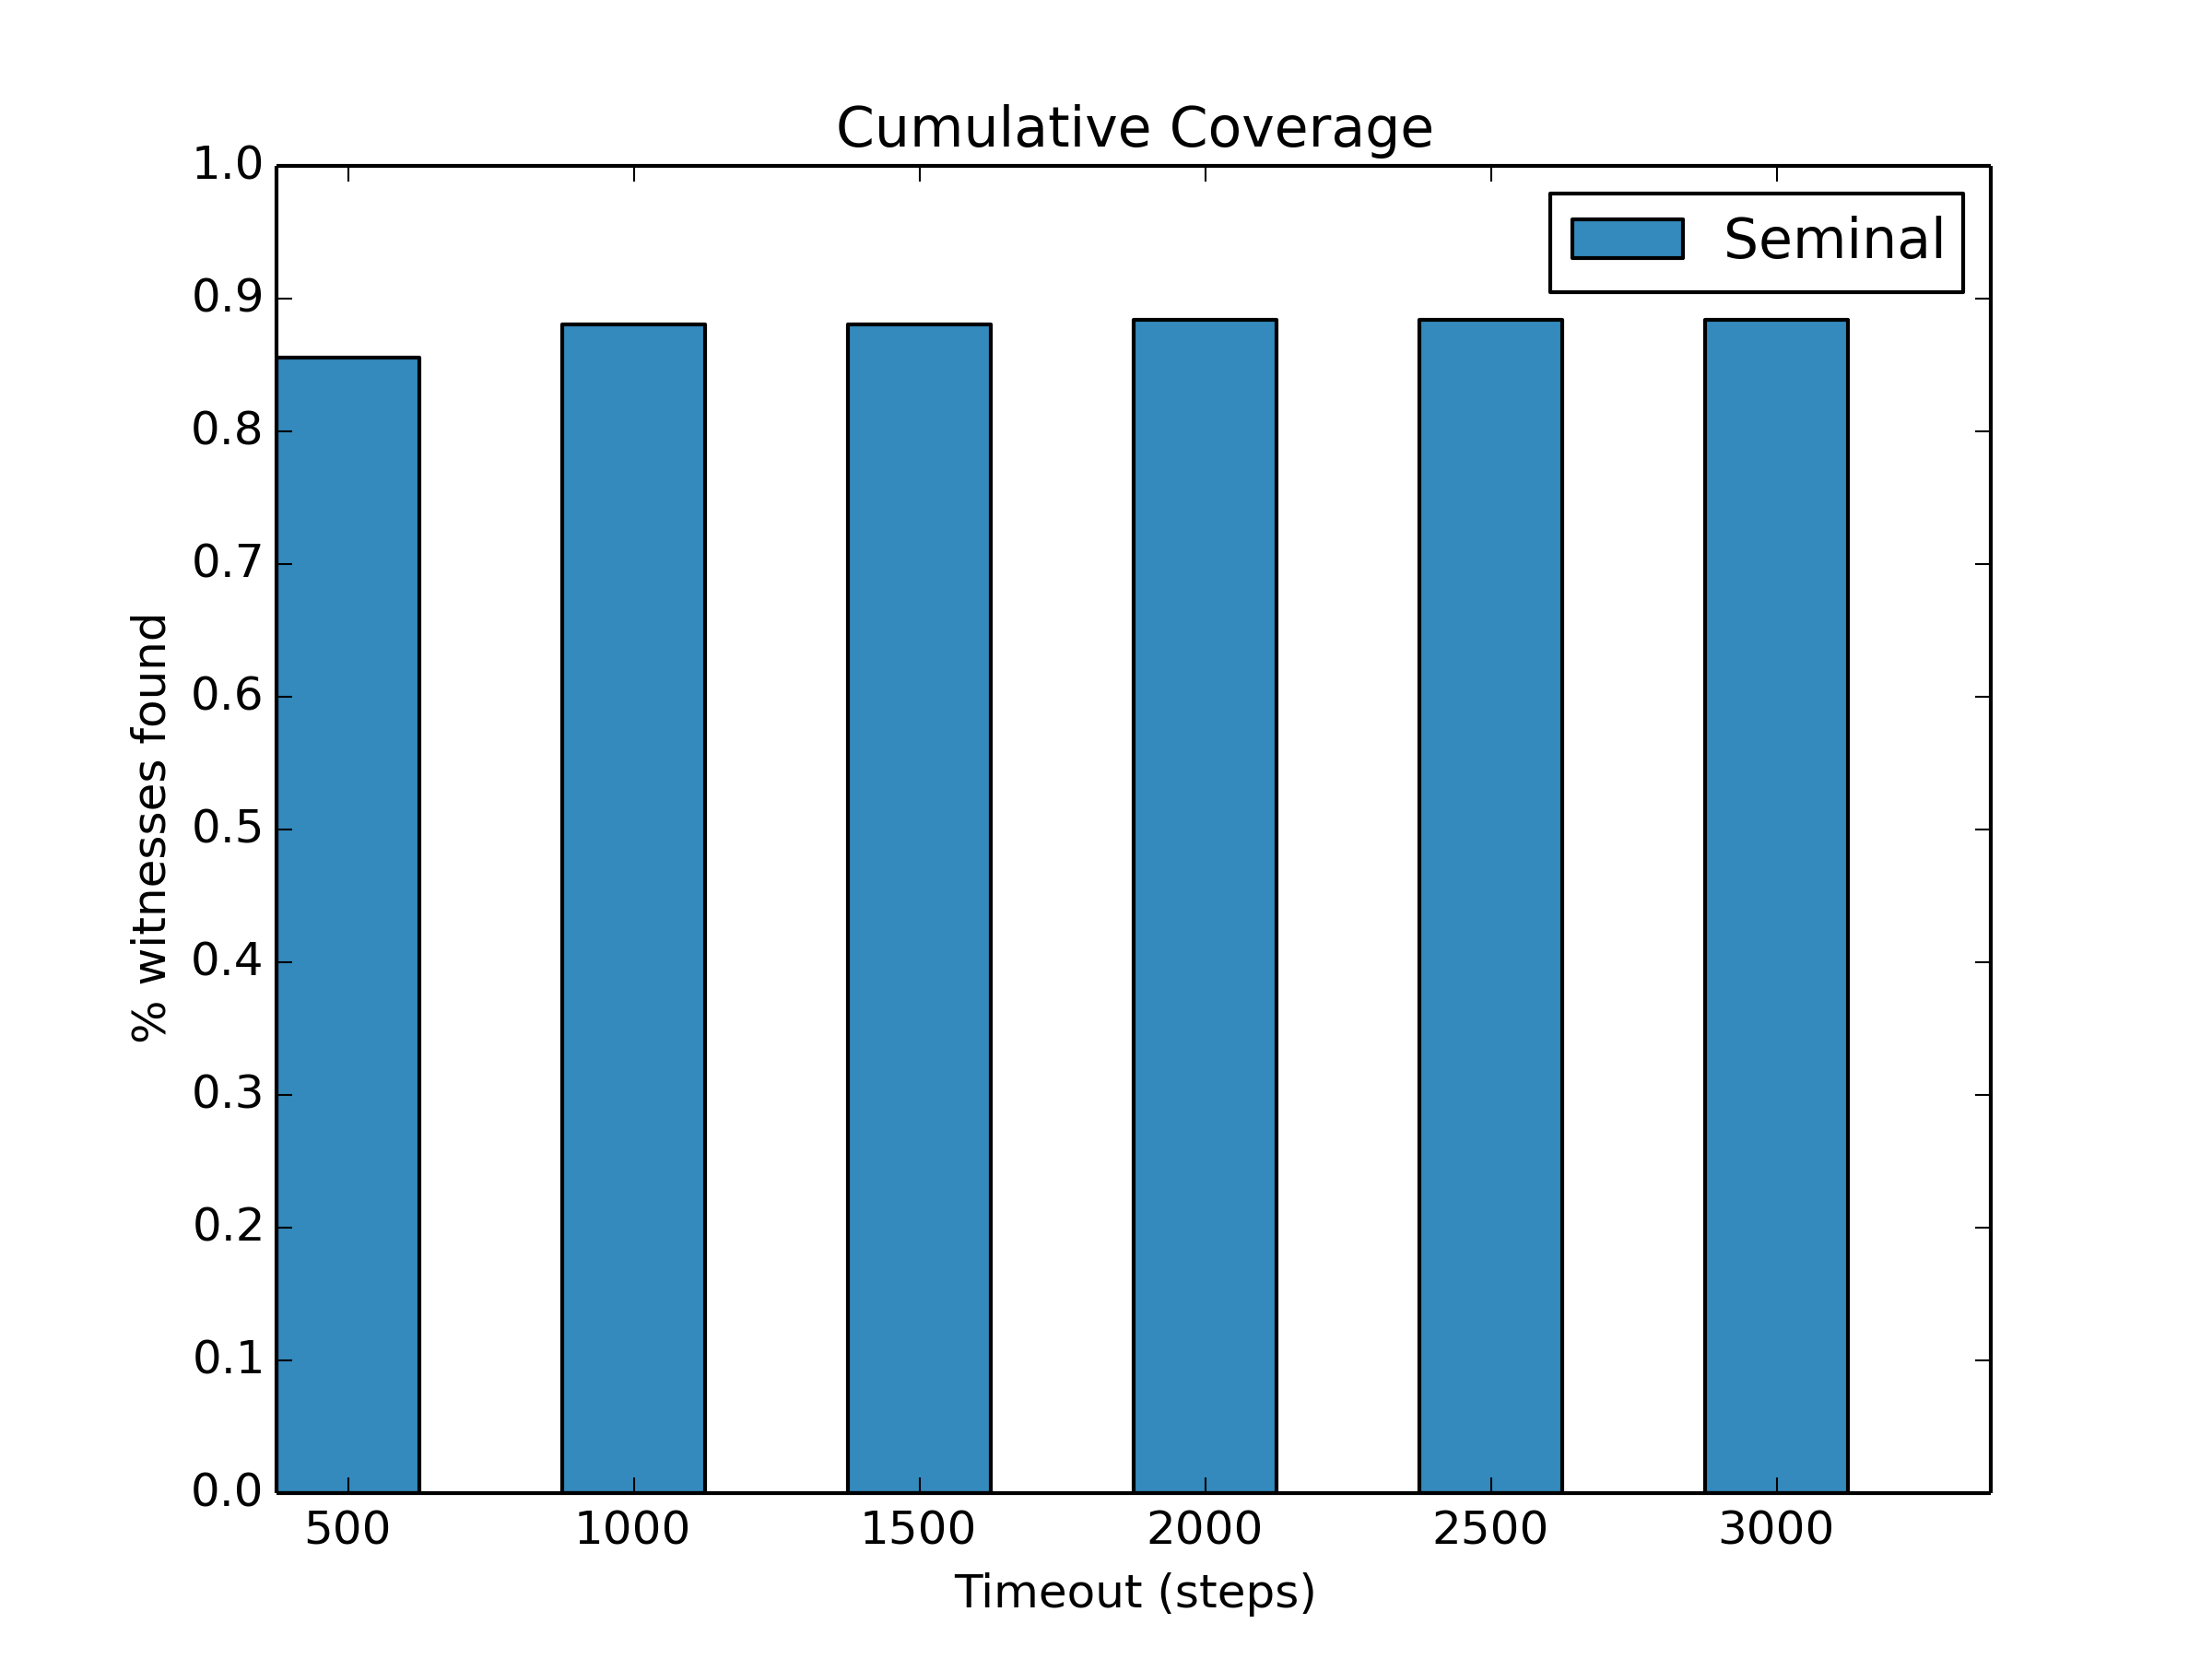
\includegraphics[width=0.49\linewidth]{coverage.png}
% \end{minipage}
% \begin{minipage}{\linewidth}
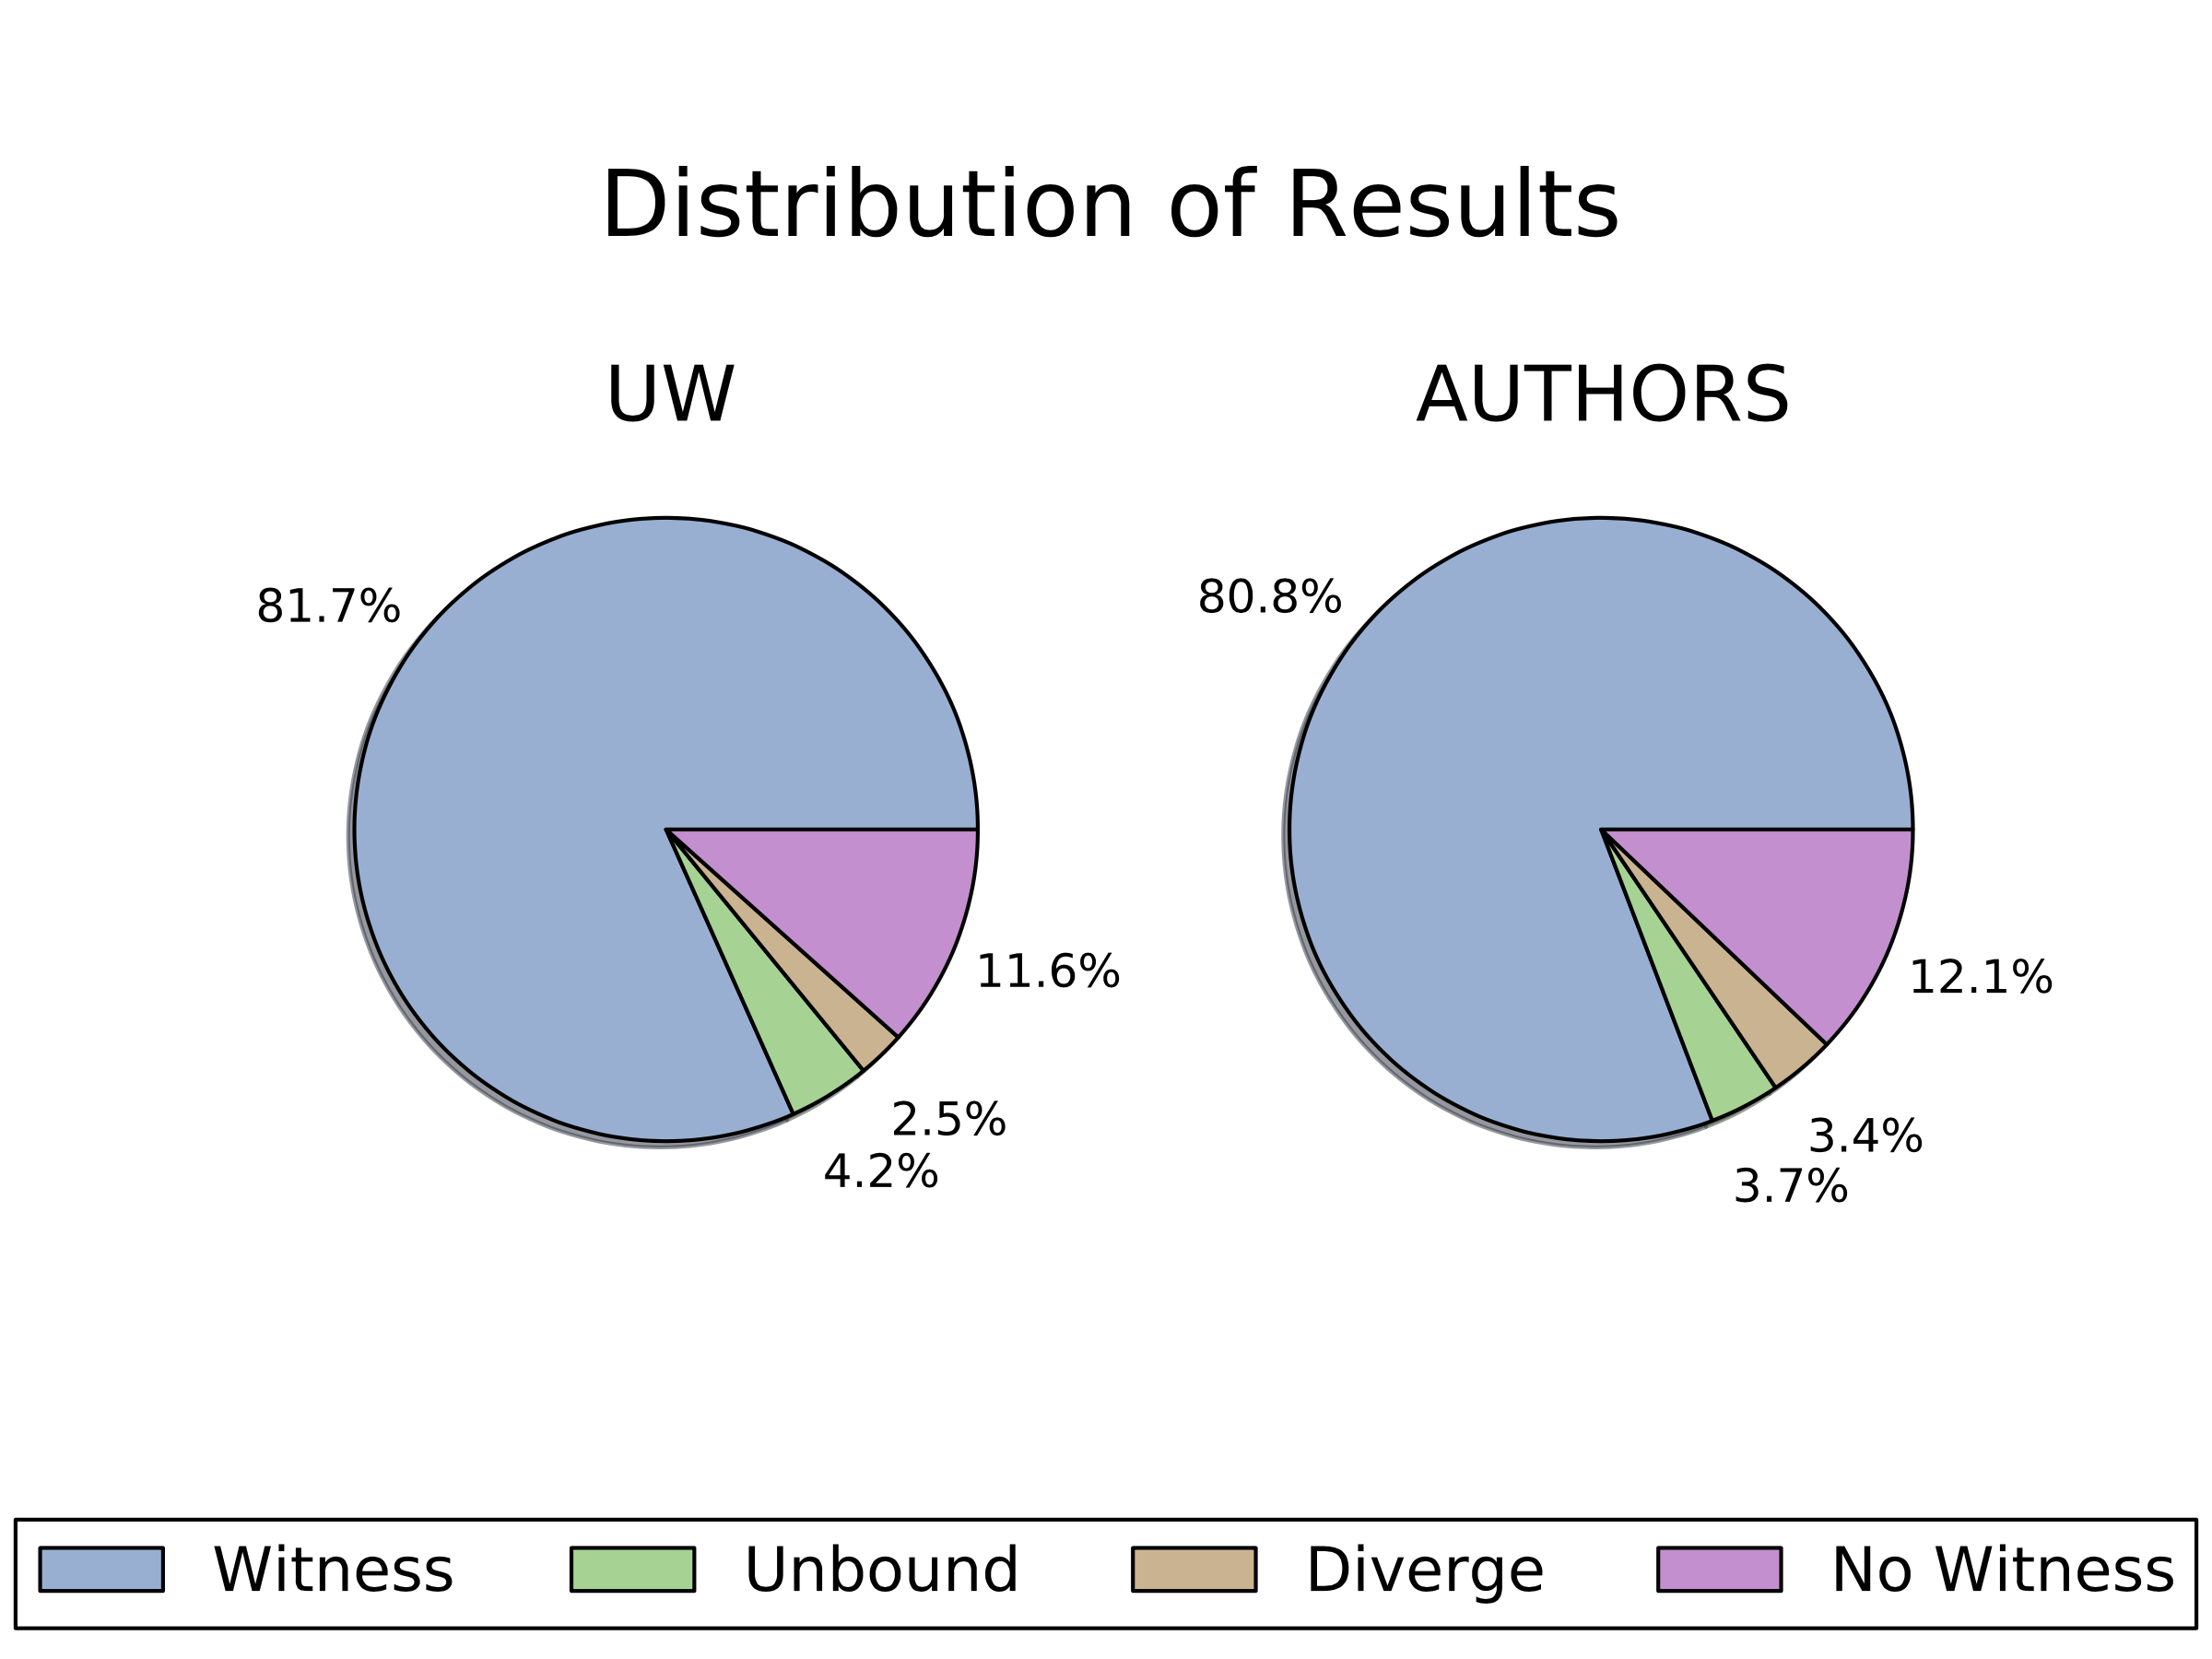
\includegraphics[width=0.49\linewidth]{distrib.png}
\end{minipage}
% \vspace{-8ex}
\caption{Results of our coverage testing and the distribution of test
  outcomes. Our random search successfully finds witnesses for 79--85\% of
  the programs in under one second, improving to 87\% in under
  10 seconds. In both datasets we detect actual type errors about 82\%
  of the time, unbound variables or constructors 3--4\% of the time, and
  diverging loops 2--3\% of the time. For the remaining 11--12\% of the
  programs we are unable to provide any useful feedback.  }
\label{fig:results-witness}
\end{figure*}

\paragraph{Results}
\label{sec:results-witness}
The results of our experiments are summarized in
Figure~\ref{fig:results-witness}.
%
In both datasets our tool was able to find a witness for 83\% of the
programs in under one second, \ie\ fast enough to be integrated as a
compile-time check. If we extend our tolerance to a 10 second timeout,
we hit a maximum of 87\% coverage.
%
Interestingly, while the vast majority of witnesses corresponded to a
type-error, as expected, 3--4\% triggered an unbound variable error (even
though \ocaml\ reported a type error) and 2--3\% triggered an infinite
recursion error.
%
For the remaining 12\% of programs we were unable to provide any useful
feedback as they either completed 1,000 tests successfully, or timed out
after one minute.
%
% XX programs were deemed safe and XX timed out even at 3,000 steps, \ie
% we could not provide any useful feedback for XX\% of the total programs.
%
While a more advanced search procedure, \eg\ dynamic-symbolic execution,
could likely trigger more of the type errors, our experiments suggest that
type errors are coarse enough (or that novice programs are \emph{simple}
enough) that these techniques are not necessary.


\subsection{Witness Complexity}
\label{sec:trace-complexity}

For each of the ill-typed programs for which we could
find a witness, we measure the complexity of the generated
trace according to two metrics.

% \paragraph{Metrics} Thus, our two metrics are:
% size of the full trace,
% \ie the number of small-step reductions, and the size of the jump-compressed
% version of the trace.
%
\begin{enumerate}
\item \emphbf{Single-step Metric} The size of the trace after expanding
  all of the single-step edges from the witness to the stuck term, and
  % This can be thought of as a worst-case
  % complexity, \ie ``How big is the fully-expanded trace?''
\item \emphbf{Jump-compressed Metric} The size of the jump-compressed trace.
\end{enumerate}


% \item \ES{others?}
%
\begin{figure*}[ht]
\centering
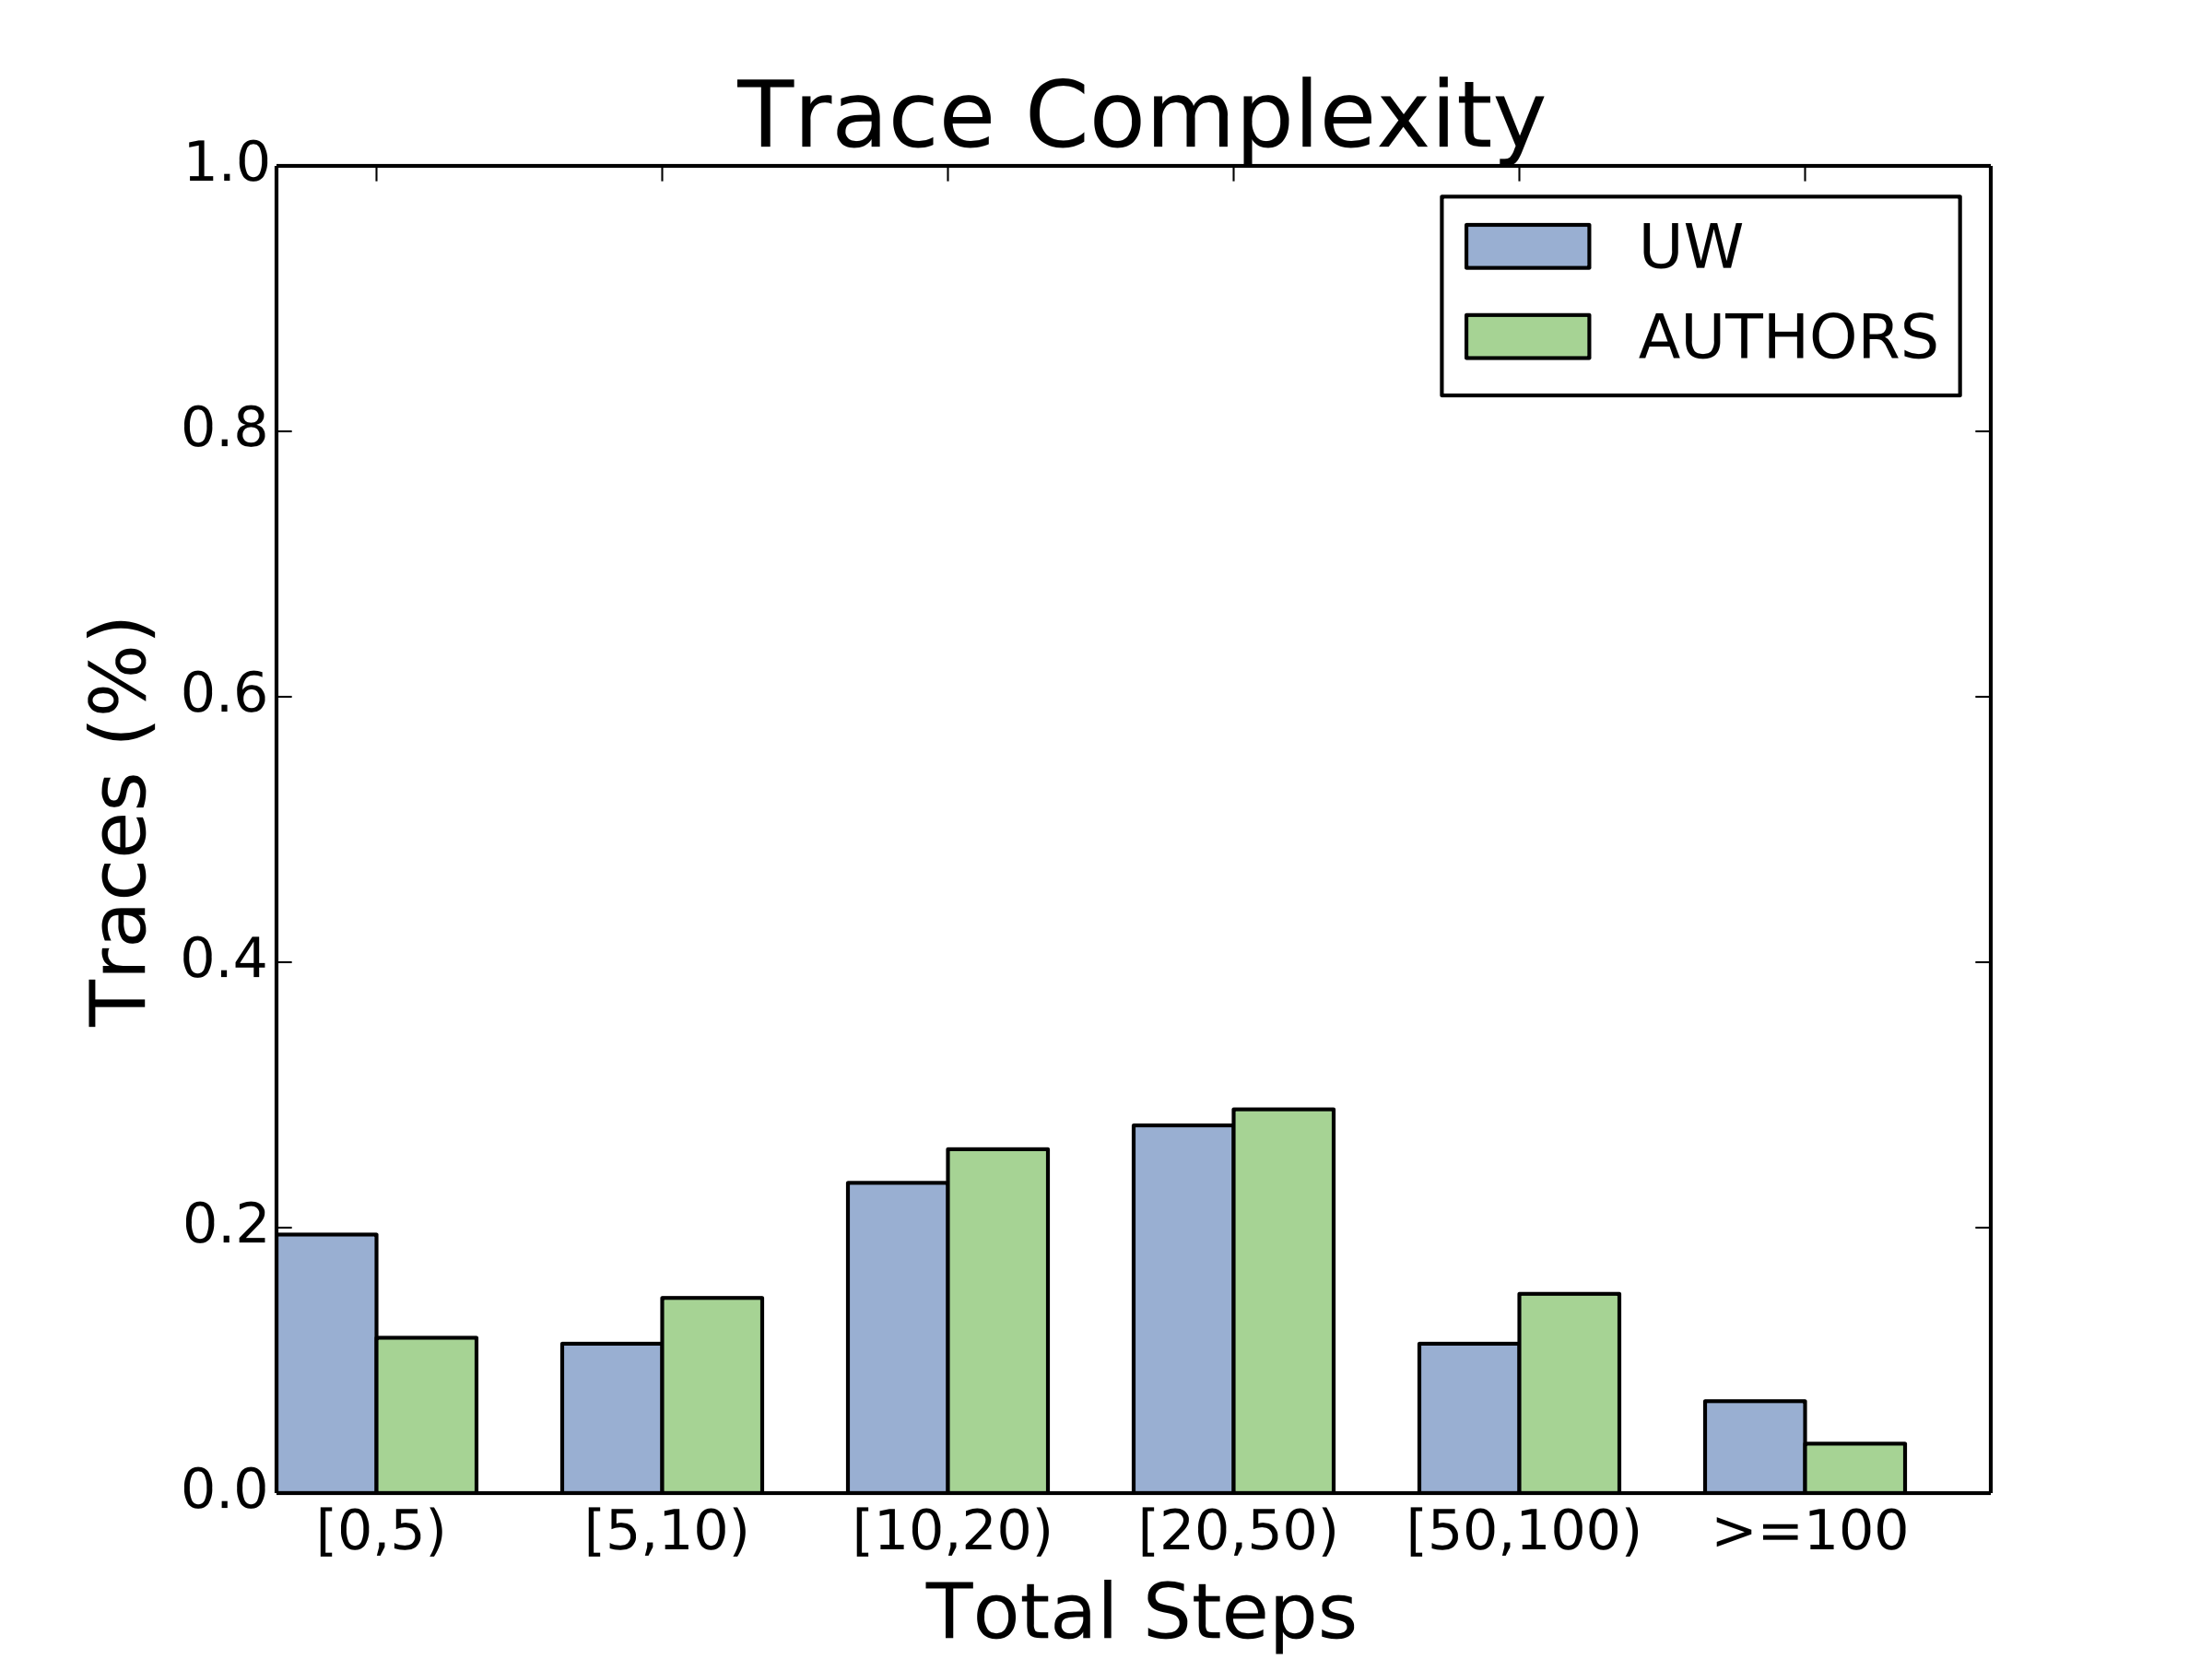
\includegraphics[width=0.49\linewidth]{trace_size_step.png}
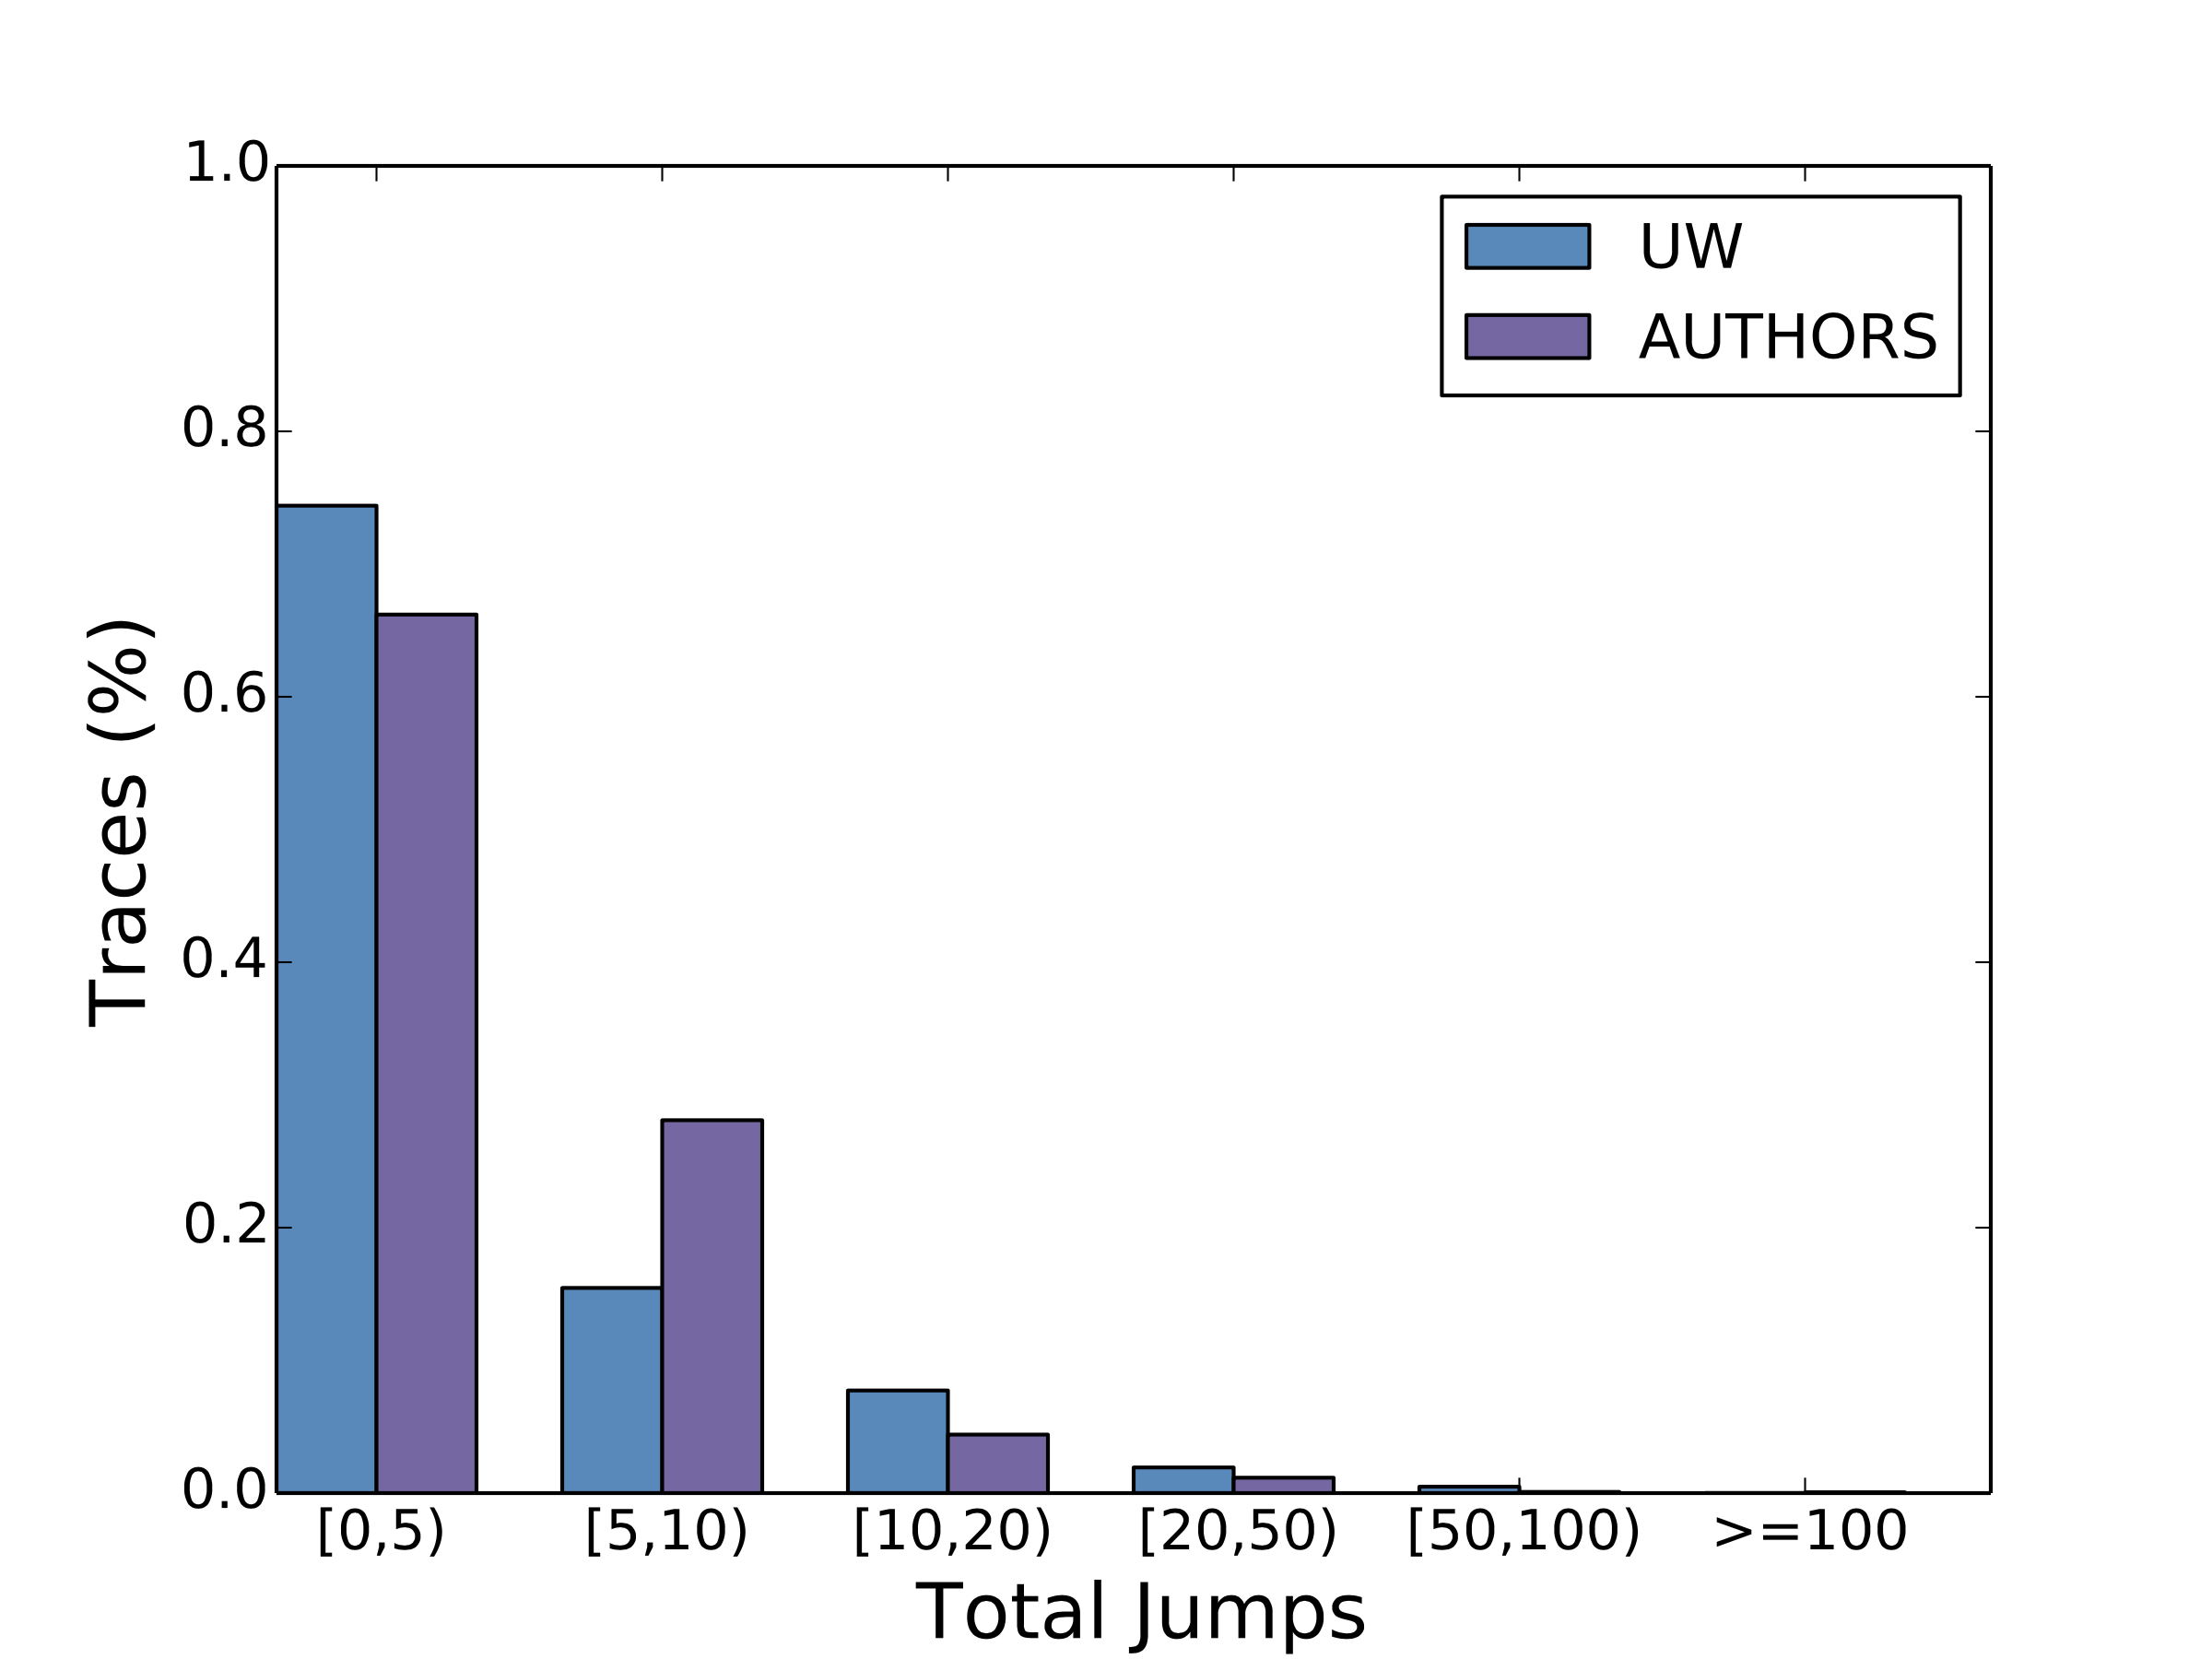
\includegraphics[width=0.49\linewidth]{trace_size_jump.png}
\caption{Complexity of the generated traces. 81\% of the combined traces
  have a jump complexity of at most 10, with an average complexity of 7
  and a median of 5.}
\label{fig:results-complexity}
\end{figure*}
%

\paragraph{Results}
\label{sec:results-complexity}
The results of the experiment are summarized in
Figure~\ref{fig:results-complexity}.
%
The average number of single-step reductions per trace is 31 for the
\ucsdbench\ dataset (35 for the \uwbench\ dataset) with a maximum of
2,745 (986 for \uwbench) and a median of 17 (also 17 for \uwbench).
%
The average number of jumps per trace is 7 (also 7 for \uwbench) with a
maximium of 353 (185 for \uwbench) and a median of 4 (also 4 for
\uwbench).
%
In both datasets 80\% or more traces have at most 10 jumps.
%


\subsection{Witness Utility}
\section{The Advantage Of Traces}\label{sec:advantage-traces}

Next, we present a \emph{qualitative} evaluation that compares
the explanations provided by \toolname's dynamic witnesses with
the static reports produced by the \ocaml\ compiler and \sherrloc,
a state-of-the-art fault localization approach~\cite{zhang_toward_2014}.
%
In particular, we illustrate, using a series of examples drawn
from student programs in the \ucsdbench\ dataset how \toolname's
jump-compressed traces can get to the heart of the error by
%
highlighting the conflicting values that cause the program to get
stuck, rather that blaming a single one,
%
showing the steps necessary to reach the stuck state, and
%
not assuming that a function is correct just because it type-checks.
%
For each example we will present
(1)~the code,
(2)~the error message returned \ocaml,
(3)~the error locations returned by \ocaml\ (underlined) and \sherrloc\ (in bold),
\footnote{When the locations from \ocaml\ and \sherrloc\ overlap,
we just underline the relevant code.}
(4)~the jump-compressed trace produced by \toolname.

% \begin{figure*}[ht]
% \centering
% \begin{minipage}{0.49\linewidth}
% \centering


\paragraph{Example: Recursion with Bad Operator}
The recursive function @sqsum@ should square each
element of the input list and then compute the sum
of the result.
%
\begin{ecode}
  let rec sqsum xs = match xs with
    | [] -> 0
    | h::t -> __(sqsum t)__ @ (h * h)
\end{ecode}
%
Unfortunately the student has used the list-append
operator |@| instead of \texttt{+} to compute the sum.
%
Both \ocaml\ and \sherrloc\ blame the \emph{wrong location},
namely the recursive call @sqsum t@ with the message
%
\begin{verbatim}
  This expression has type
    int
  but an expression was expected of type
    'a list
\end{verbatim}
%
\toolname\ produces the following trace showing how the evaluation of
@sqsum [1]@ gets stuck:
%
\begin{center}
  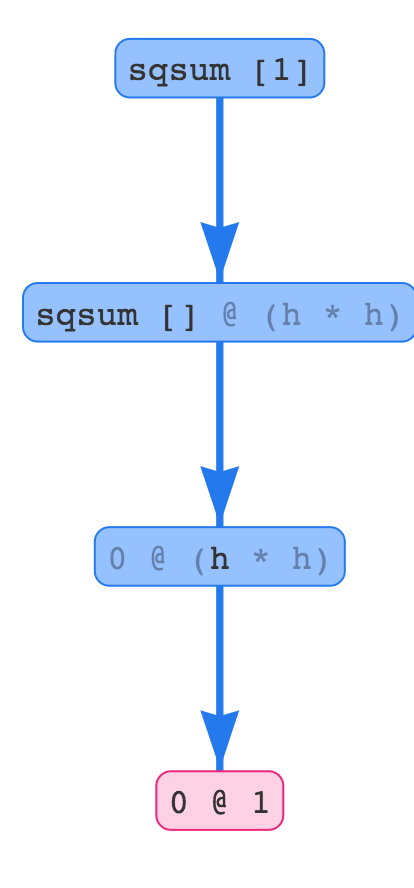
\includegraphics[height=125px]{sqsum.png}
\end{center}
%
The figure highlights the entire stuck term
(not just the recursive call), emphasizing
the \emph{conflict} between @int@ and @list@
rather than assuming one or the other is correct.

\paragraph{Example: Recursion with Bad Base Case}
%
The function @sumList@ should add up
the elements of its input list.
%
\begin{ecode}
  let rec sumList xs = match xs with
    | []    -> ==[]==
    | y::ys -> y + __sumList ys__
\end{ecode}
%
Unfortunately, in the base case, it returns @[]@
instead of @0@.
%
\sherrloc\ blames the base case, and \ocaml\
assumes the base case is correct and blames
the \emph{recursive call} on line 3:
%
\begin{verbatim}
  This expression has type
    'a list
  but an expression was expected of type
    int
\end{verbatim}
%
Both of the above are parts of the full story, which
is succinctly summarized by \toolname's trace showing
how @sumList [1; 2]@ gets stuck at @2 + []@.
%
\begin{center}
  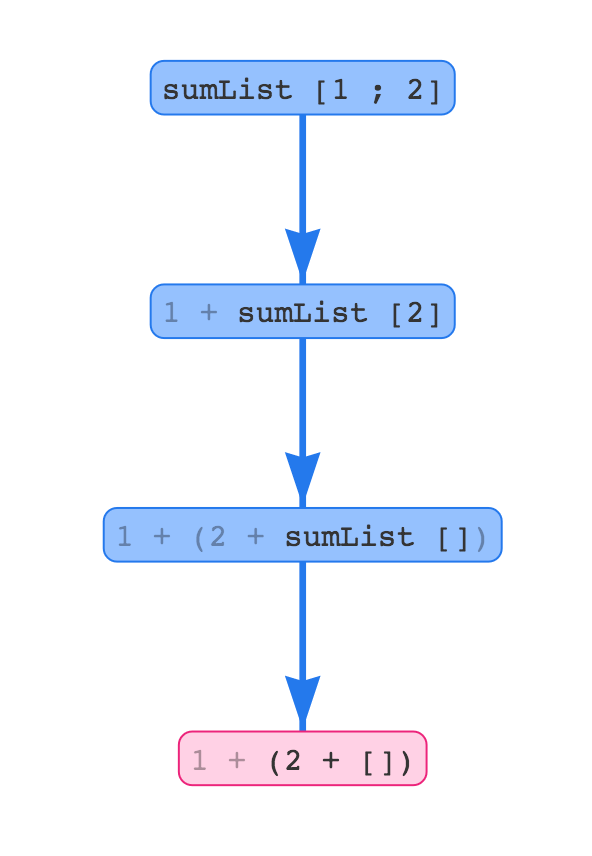
\includegraphics[height=125px]{sumlist.png}
\end{center}
%
The trace clarifies immediately (via the third step)
that the @[]@ is the result of the recursive call
@sumList []@, and shows how it is incompatible with
the subsequent \texttt{+} operation.

%% ES: append is actually a bit problematic as we don't find the nice
%% append [1] [2] witness. instead we could find something like
%% append [_] [], but it's not as clear IMO
% Our next example is the @append@ function, which should concatenate the
% two input lists.
% %
% \begin{ecode}
% let append xs ys = match xs with
%   | []   -> ys
%   | h::t -> h :: __t__ :: ys
% \end{ecode}
% %
% The student has forgotten to make a recursive call to @append@, and
% instead tries to cons the tail @t@ directly onto the second list @ys@.
% Consing @h@ back onto the result causes \ocaml to attempt to construct
% the infinite type @'a = 'a list@, triggering an \emph{occurs-check}
% error.
% %
% \begin{verbatim}
% Error: This expression has type
%          'a list
%        but an expression was expected of type
%          'a
%        The type variable 'a occurs inside 'a list
% \end{verbatim}
% %
% %
% \begin{center}
%   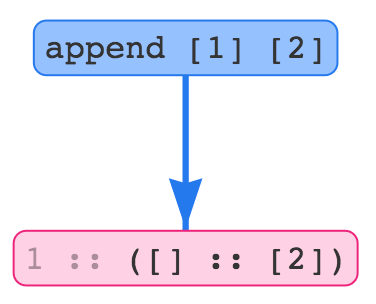
\includegraphics[height=75px]{append.png}
% \end{center}

\paragraph{Example: Bad Helper Function that Type-Checks}
%
The function @digitsOfInt@ is supposed to return a list of
the digits of the input integer.
%
\begin{ecode}
  let append x xs =
    match xs with
    | [] -> [x]
    | _  -> x :: xs

  let rec digitsOfInt n =
    if n <= 0 then
      []
    else
      append (==digitsOfInt (n / 10)==)
             [__n mod 10__]
\end{ecode}
%
Unfortunately, the student's @append@ function \emph{conses} an element
onto a list instead of appending two lists.
%
Though incorrect, @append@ still type-checks and thus \ocaml and
\sherrloc blame the \emph{use-site} on line 10.
%
\begin{verbatim}
  This expression has type
    int
  but an expression was expected of type
    'a list
\end{verbatim}
%
\toolname, in contrast, makes no asummptions about @append@ and produces
a trace that illustrates the true error on line 4, by
highlighting the conflict in consing a list onto a list of integers.
%
\begin{center}
  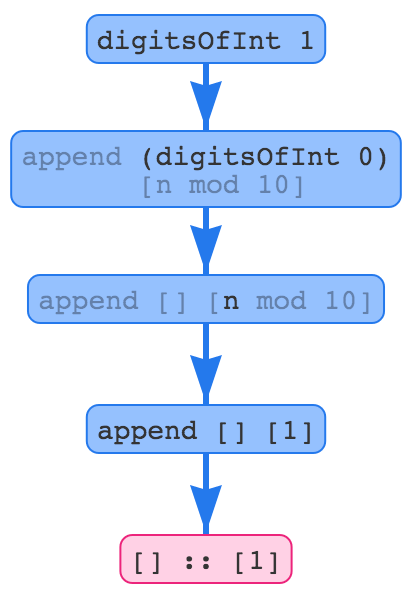
\includegraphics[height=175px]{digitsOfInt.png}
\end{center}
%

\paragraph{Example: Higher-Order Functions}
%
The higher-order function @wwhile@ is supposed
to emulate a traditional while-loop. It takes
a function @f@ and repeatedly calls @f@ on the
first element of its output pair, starting with
the initial value @b@, until the second element
is @false@.
%
\begin{ecode}
  let rec wwhile (f,b) =
    match f with
    | (z, false) -> z
    | (z, true)  -> wwhile (f, z)

  let f x =
    let xx = x * x in
    (xx, (xx < 100))

  let _ = wwhile (__f__, 2)
\end{ecode}
%
Unfortunately, the student has forgotten to \emph{apply}
@f@ at all on line 2, and just matches it directly against
a pair.
This faulty definition of @wwhile@ still typechecks however,
and hence, are ``assumed'' to be correct by and both \ocaml\
and \sherrloc\ which blame the \emph{use-site} on line 10.
%
\begin{verbatim}
  This expression has type
    int -> int * bool
  but an expression was expected of type
    'a * bool
\end{verbatim}
%
\toolname\ synthesizes a trace that draws the eye to the
true error: the @match@ expression on line 2, and highlights
the conflict in matching a function against a pair pattern.
%
\begin{center}
  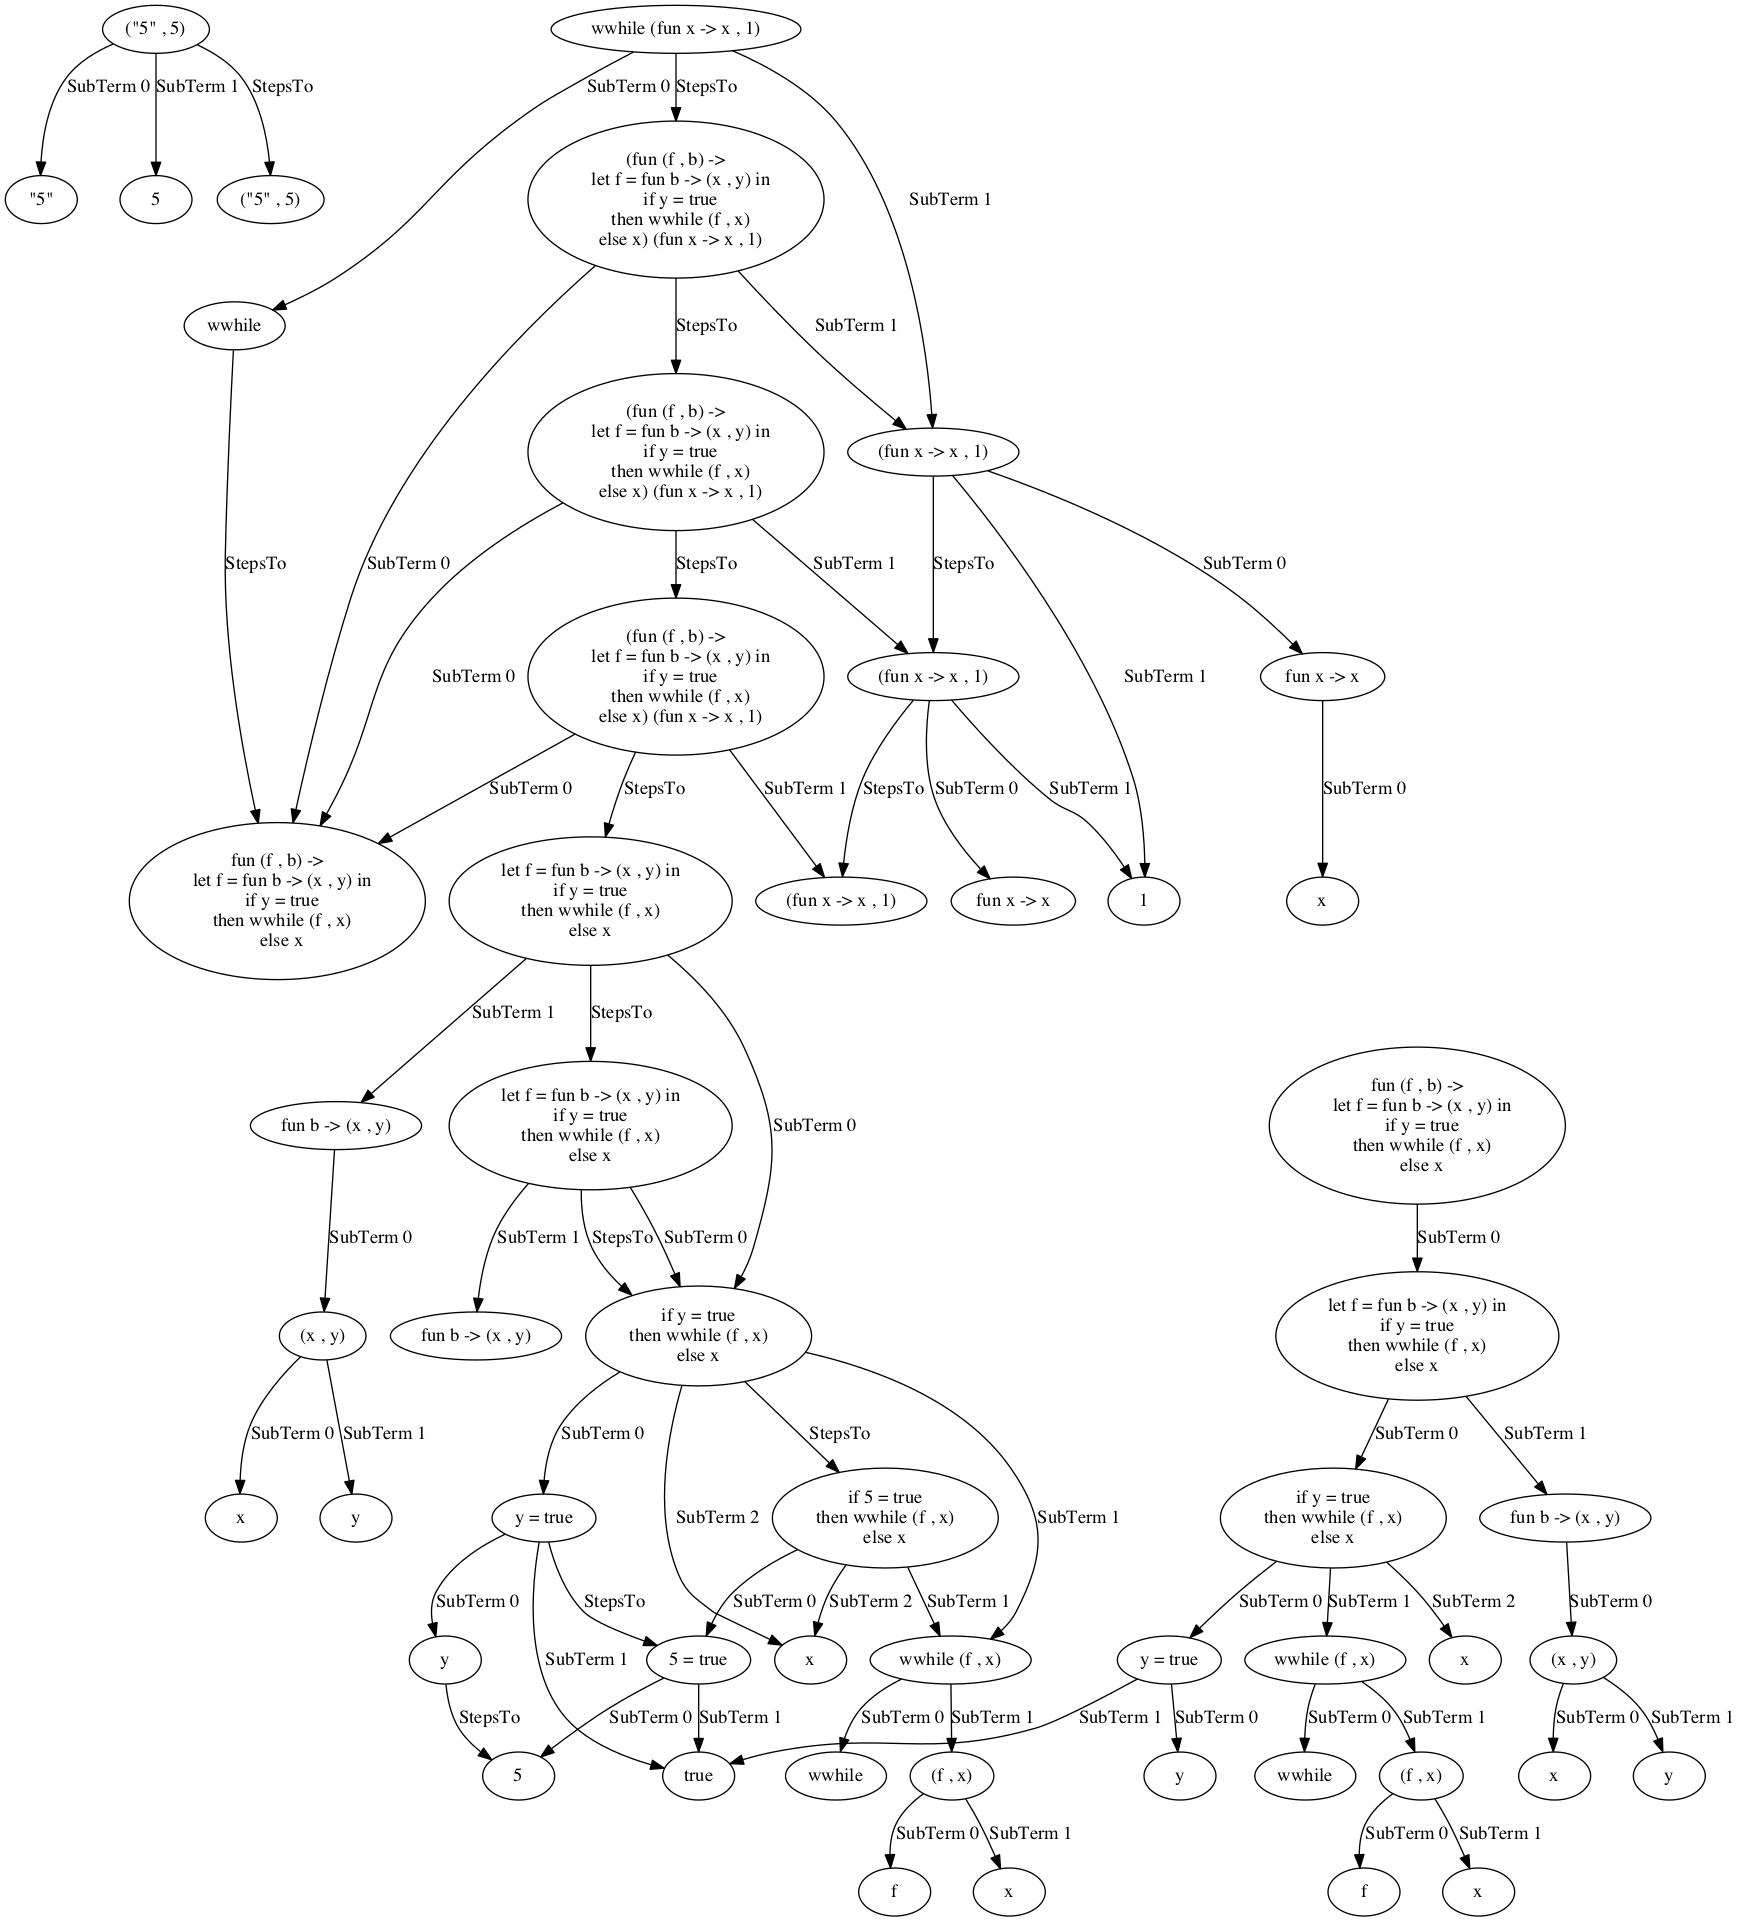
\includegraphics[height=150px]{wwhile.png}
\end{center}
%
By highlighting conflicting values (\ie\ the source and sink
of the problem) and not making any assumptions, \toolname\
focusses the user's attention on the piece of code that is
actually relevant to the error.


%%% Local Variables:
%%% mode: latex
%%% TeX-master: "main"
%%% End:


\subsubsection{Quantitative}
\label{sec:user-study}
% Finally, to test the explanatory power of our jump-compressed traces, we
% ran a user study (IRB \#2014009900) at the University of Virginia (UVA).
% %
% We included four problems in an exam in the Spring session of UVA's
% undergraduate Programming Languages course (CS 4501).
% %
% We presented the 60 students in the course with ill-typed \ocaml\
% programs and asked them to
% %
% (1) \emph{explain} the type error, and
% %
% (2) \emph{fix} the type error.
% %
% For each problem the student was given the ill-typed program and
% either \ocaml's error message or \toolname's jump-compressed trace.
%
We assigned four problems to the ($n=60$) students in the course: the
@sumList@, @digitsOfInt@, and @wwhile@ programs from
\S~\ref{sec:advantage-traces}, as well as the following @append@ program
%
\begin{ecode}
  let append x l =
    match x with
    | []   -> l
    | h::t -> h :: t :: l
\end{ecode}
%
which triggers an occurs-check error on line 4.
%
For each problem the students were given the ill-typed program and
either \ocaml's error message or \toolname's jump-compressed trace.
%
Due to the nature of an in-class exam, not every student answered every
question; we received between 13 and 28 (out of a possible 30) responses
for each problem-tool pair.

We then instructed four annotators (one of whom is an author, the other
three are teaching assistants at UCSD) to classify the answers as
correct or incorrect.
%
We performed an inter-rater reliability (IRR) analysis to determine the
degree to which the annotators consistently graded the exams.
%
As we had more than two annotators assigning nominal (``correct'' or
``incorrect'') ratings we used Fleiss' kappa~\cite{Fleiss1971-du} to
measure IRR.\@
%
Fleiss' kappa is measured on a scale from $1$, indicating total
agreement, to $-1$, indicating total disagreement, with $0$ indicating
random agreement.

\paragraph{Threats to Validity}
\subparagraph{Construct}
%
Measuring understanding is a difficult task; we used the correctness of
the student's explanation of, and fix for, the type error as a proxy for
her understanding, but it is possible that other metrics would produce
different results.

\subparagraph{Internal}
%
We assigned students randomly to two groups. The first group was given
\ocaml's errors for @append@ and \hbox{@digitsOfInt@,} and \toolname's trace
for @sumList@ and @wwhile@. The second group was given the opposite
assignment of errors and traces. This assignment ensured that (1) each
student was given \ocaml and \toolname problems, and (2) each student
was given an ``easy'' and ``hard'' problem for both \ocaml and
\toolname. Students without sufficient knowledge of \ocaml could affect
the results, as could the time-constrained nature of an exam. For these
reasons we excluded any answers left blank from our analysis.

\subparagraph{External}
%
Our experiment is based on students in the process of learning \ocaml,
and thus may not generalize to all developers. The four
programs we used were chosen manually, via a random selection and
filtering of the programs in the \ucsdbench dataset. In some cases we made
minor simplifying edits (\eg alpha-renaming, dead-code removal) to the
programs to make them more understandable in the short timeframe of an
exam; however, we never altered the resulting type-error. A different
selection of programs may lead to different results.

\subparagraph{Conclusion}
%
We collected exams from 60 students, though due to the nature of the
study not every student completed every problem.
%
The number of complete submissions ranges from 13 (for the \toolname
version of @wwhile@) to 28 (for the \ocaml version of @sumList@), out of
a maximum of 30 per program-tool pair.
%
Collecting more responses per test pair was not possible, as it
would require having students answer the same problem twice (once with
\ocaml and once with \toolname).


\paragraph{Results}
%
Figure~\ref{fig:results-user-study} summarizes a single annotator's
results, which show that students given \toolname's jump-compressed
trace were consistently more likely to correctly explain
and fix the type error than those given \ocaml's error message.
%
Across each problem the \toolname responses were marked correct
$10-30\%$ more often than the \ocaml responses, which suggests that
the students who had access to \toolname's traces had a better
understanding of the type errors.
%
The measured kappa values were $\kappa = 0.72$ for the explanations and
$\kappa = 0.83$ for the fixes; while there is no formal notion for what
consititutes strong agreement~\cite{Krippendorff2012-wd}, kappa values
above $0.60$ are often called ``substantial''
agreement~\cite{Landis1977-ey}.
%
\begin{figure*}[ht]
\centering
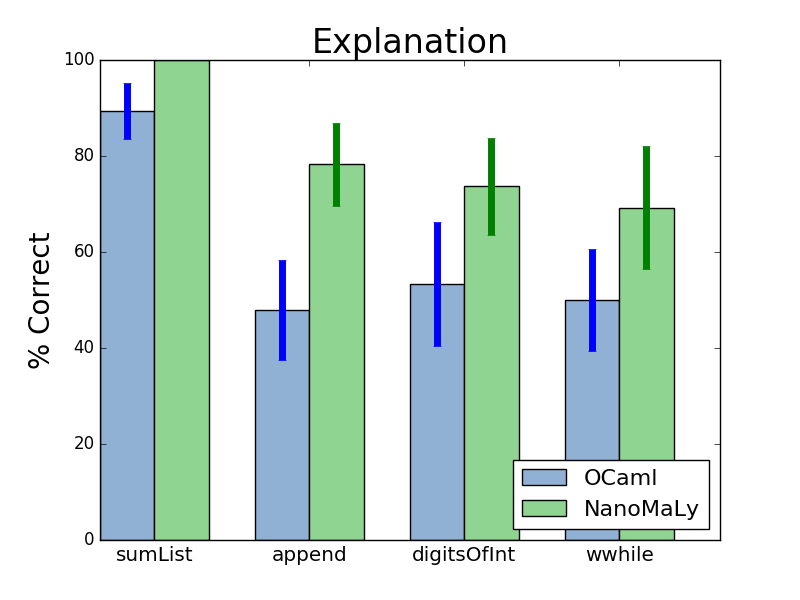
\includegraphics[width=0.49\linewidth]{user-study-reason.png}
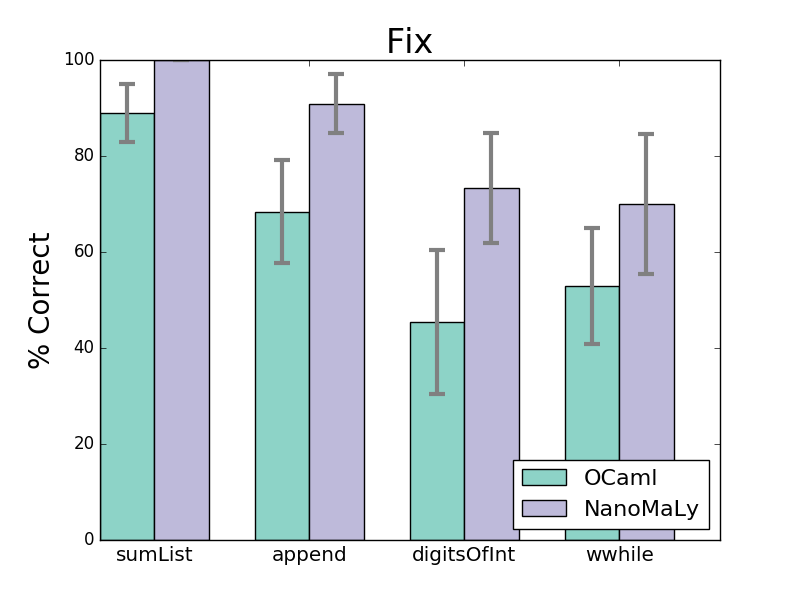
\includegraphics[width=0.49\linewidth]{user-study-fix.png}
\caption{A classification of students' explanations and fixes for type
  errors, given either \ocaml's error % message
  or \toolname's
  jump-compressed trace. The students given \toolname's jump-compressed
  trace consistently scored better ($\ge 10\%$) than those given \ocaml's type
  error.}
\label{fig:results-user-study}
\end{figure*}
%

\subsection{Discussion}
\label{sec:discussion}

To summarize, our experiments demonstrate that \nanomaly finds witnesses
to type errors: (1) with high coverage in a timespan amenable to
compile-time analysis, (2) with traces that have a low average
complexity of 7 jumps, and (3) that are more helpful to novice
programmers than traditional type error messages.

There are, of course, drawbacks to our approach. Four that stand out
are: (1) coverage limits due to random generation, (2) the inability to
handle certain instances of infinite types, (3) dealing with an
explosion in the size of generated traces, and (4) handling ad-hoc
polymorphism.

\paragraph{Random Generation}
Random test generation has difficulty generating highly constrained
values, \eg\ red-black trees or a pair of equal integers. If the type
error is hidden behind a complex branch condition \nanomaly\ may not be
able to trigger it. Exhaustive testing and dynamic-symbolic execution
can address this short-coming by performing an exhaustive search for
inputs (\emph{resp}.\ paths through the program). As our experiments
show, however, novice programs do not appear to require more advanced
search techniques, likely because the novice programs tend to be simple.

\paragraph{Infinite Types}
Our implementation does check for infinite types inside \forcesym, but
there are some degenerate cases where it is unable to detect
them. Consider, the following buggy @replicate@
%
\begin{code}
  let rec replicate n x =
    if n <= 0 then
      []
    else
      replicate (n-1) [x]
\end{code}
%
This code produces a nested list (with @n@ levels of nesting) containing
a single copy of @x@, instead of a list with @n@ copies of @x@. \ocaml\
detects a cyclic \hbox{@'a = 'a list@} constraint in the recursive call
and throws a type error, whereas \nanomaly\ happily % recurses @n@ times to
produces the nested list.  Strictly speaking, this function itself cannot
``go wrong'', the program would not get stuck until a \emph{client}
attempted to use the result expecting a flat list. But this is not very
satisfying as @replicate@ is clearly to blame. Furthermore, in our
experience, infinite-type errors are often difficult to %some of the more difficult ones to
debug (and to explain to novices), so better support for this scenario
would be useful.

\paragraph{Trace Explosion}
Though the average complexity of our generated traces is low in terms of
jumps, there are some extreme outliers.
%
We cannot reasonably expect a novice user to explore a trace containing
50+ terms and draw a conclusion about which pieces contributed to the
bug in their program.
%
Enhancing our visualization to slice out program paths relevant to
specific values~\cite{Perera2012-dy}, would likely help alleviate this
issue, allowing users to highlight a confusing value and ask: ``Where
did this come from?''

\paragraph{Ad-hoc Polymorphism}
Our approach can only support ad-hoc polymorphism (\eg\ type-classes in
\haskell\ or polymorphic comparison functions in \ocaml) in limited cases
where we have enough typing information at the call-site to resolve the
overloading. For example, consider the @n <= 0@ test in our @fac@ example.
@<=@ is polymorphic in \ocaml, but in this case we can make progress because
the literal @0@ is not. If we parameterized @fac@ by a lower bound, \eg
%
\begin{code}
  let rec fac n m =
    if n <= m then
      1
    else
      n * fac (n - 1) m
\end{code}
%
and called @fac@ with two holes, we would get stuck at the @n <= m@
test; not because of a type error, but because all we know about
@n@ and @m@ at that point is that they must have the same (unknown)
type.

This issue is uncommon in \ocaml\ (we did not detect a single instance
of it across all of our benchmarks), but it would surely be exacerbated
by a language like \haskell, which makes heavy use of overloading. We
suspect that dynamic-symbolic execution would allow us to handle ad-hoc
polymorphism, but defer a proper treatment to future work.

% \begin{itemize}
% \item benchmarks: our data + seminal data
% \item both cases: \textbf{random} search sufficient to trigger runtime crash in 80\% of programs
% \item how many of the ``safe'' programs are actually safe??
% \end{itemize}

%%% Local Variables:
%%% mode: latex
%%% TeX-master: "main"
%%% End:
%!TEX root = main.tex



\item values are tagged with their types, just like ``untyped'' langs
\item special ``hole'' value whose type is not yet known, used for function args
\item on-the-fly unification to determine ``correct'' type for holes
\end{itemize}

% Algorithm:
%   Input: ML Program (let f1 = e1 in let f2 = e2 in ... e)
%   Output: 'safe' or 'fn v1 .. vn' where 'fn v1 .. vn' gets stuck

